\newcommand{\packedTagResultsAucTable}{
    \begin{table}[H]
        \centering
        \begin{tabular}{|p{2,8cm}||p{2,8cm} p{2,8cm} p{2,8cm}|}
            \hline
            Packed Tag & ALOHA & Joint Embedding & Proposed Model \\
            \hline
            AUC-ROC & 0.593$\pm$0.052 & 0.531$\pm$0.062 & \textBF{0.607$\pm$0.142} \\
            \hline
        \end{tabular}
        \caption{AUC-ROC (Area Under Curve) of the different models for the \textbf{Packed Tag} prediction task. Results were aggregated over \textBF{3} training runs with different weight initializations and minibatch orderings. Best results are shown in \textbf{bold}.} \label{tab:packedTag_auc}
    \end{table}
}

\newcommand{\packedTagResultsAtFprTable}{
    \begin{center}
        \begin{longtable}[c]{|p{3,2cm}||p{1,8cm} p{1,8cm} p{1,8cm} p{1,8cm} p{1,8cm}|}
            \hline
            Packed Tag & \multicolumn{5}{c|}{{FPR}} \\
            & $10^{-5}$ & $10^{-4}$ & $10^{-3}$ & $10^{-2}$ & $10^{-1}$ \\
            \hline
            \endfirsthead

            \caption*{\raggedright ...continued from previous page} \\
            \hline
            Packed Tag & \multicolumn{5}{c|}{\textbf{FPR}} \\
            & $10^{-5}$ & $10^{-4}$ & $10^{-3}$ & $10^{-2}$ & $10^{-1}$ \\
            \hline
            \endhead

            \caption*{\raggedleft ...continued on next page} \\
            \endfoot

            \caption{Mean and standard deviation results (TPR, Accuracy, Recall, Precision and F1-Score) of the different models for the \textbf{Packed Tag} prediction task at different \textbf{FPR}s (\textit{False Positive Rates}). Results were aggregated over \textBF{3} training runs with different weight initializations and minibatch orderings. Best results are shown in \textbf{bold}. Under \textbf{TPR} results are also presented the percentage reduction in mean detection error and in ROC curve standard deviation introduced by the \textit{Proposed Model} with respect to both \textit{ALOHA} model and \textit{Joint Embedding}.} \label{tab:packedTag_results_at_fpr} \\
            \endlastfoot

            \multicolumn{6}{|c|}{\textbf{TPR}} \\
            \hline
            ALOHA & \textBF{0.000$\pm$0.000} & \textBF{0.000$\pm$0.000} & 0.006$\pm$0.008 & 0.044$\pm$0.031 & 0.136$\pm$0.110 \\
            Joint Embedding & \textBF{0.000$\pm$0.000} & \textBF{0.000$\pm$0.000} & 0.000$\pm$0.000 & \textBF{0.077$\pm$0.022} & 0.162$\pm$0.034 \\
            Proposed Model & \textBF{0.000$\pm$0.000} & \textBF{0.000$\pm$0.000} & \textBF{0.018$\pm$0.013} & 0.044$\pm$0.016 & \textBF{0.209$\pm$0.111} \\
            \hline
            Error Reduction wrt \newline ALOHA & 0.0\% & 0.0\% & 1.2\% & 0.0\% & 8.4\% \\
            Error Reduction wrt \newline Joint Embedding & 0.0\% & 0.0\% & 1.8\% & -3.6\% & 5.6\% \\
            \hline
            Std Reduction wrt \newline ALOHA & 0.0\% & 0.0\% & -62.5\% & 48.4\% & -0.9\% \\
            Std Reduction wrt \newline Joint Embedding & 0.0\% & 0.0\% & 0.0\% & 27.3\% & -226.5\% \\
            \hline
            \multicolumn{6}{|c|}{\textbf{Accuracy}} \\
            \hline
            ALOHA & \textBF{0.881$\pm$0.000} & \textBF{0.881$\pm$0.000} & 0.882$\pm$0.001 & 0.876$\pm$0.005 & 0.808$\pm$0.014 \\
            Joint Embedding & \textBF{0.881$\pm$0.000} & \textBF{0.881$\pm$0.000} & 0.881$\pm$0.000 & \textBF{0.882$\pm$0.003} & 0.812$\pm$0.004 \\
            Proposed Model & \textBF{0.881$\pm$0.000} & \textBF{0.881$\pm$0.000} & \textBF{0.883$\pm$0.001} & 0.878$\pm$0.003 & \textBF{0.817$\pm$0.015} \\
            \hline
            \multicolumn{6}{|c|}{\textbf{Recall}} \\
            \hline
            ALOHA & \textBF{0.000$\pm$0.000} & \textBF{0.000$\pm$0.000} & 0.006$\pm$0.008 & 0.044$\pm$0.031 & 0.136$\pm$0.110 \\
            Joint Embedding & \textBF{0.000$\pm$0.000} & \textBF{0.000$\pm$0.000} & 0.000$\pm$0.000 & \textBF{0.077$\pm$0.022} & 0.162$\pm$0.034 \\
            Proposed Model & \textBF{0.000$\pm$0.000} & \textBF{0.000$\pm$0.000} & \textBF{0.018$\pm$0.013} & 0.044$\pm$0.016 & \textBF{0.209$\pm$0.111} \\
            \hline
            \multicolumn{6}{|c|}{\textbf{Precision}} \\
            \hline
            ALOHA & \textBF{1.000$\pm$0.000} & \textBF{1.000$\pm$0.000} & 0.238$\pm$0.337 & 0.301$\pm$0.193 & 0.141$\pm$0.101 \\
            Joint Embedding & \textBF{1.000$\pm$0.000} & \textBF{1.000$\pm$0.000} & 0.000$\pm$0.000 & \textBF{0.505$\pm$0.079} & 0.177$\pm$0.031 \\
            Proposed Model & \textBF{1.000$\pm$0.000} & \textBF{1.000$\pm$0.000} & \textBF{0.563$\pm$0.400} & 0.358$\pm$0.094 & \textBF{0.209$\pm$0.089} \\
            \hline
            \multicolumn{6}{|c|}{\textbf{F1 Score}} \\
            \hline
            ALOHA & \textBF{0.000$\pm$0.000} & \textBF{0.000$\pm$0.000} & 0.011$\pm$0.016 & 0.076$\pm$0.053 & 0.138$\pm$0.106 \\
            Joint Embedding & \textBF{0.000$\pm$0.000} & \textBF{0.000$\pm$0.000} & 0.000$\pm$0.000 & \textBF{0.133$\pm$0.035} & 0.169$\pm$0.033 \\
            Proposed Model & \textBF{0.000$\pm$0.000} & \textBF{0.000$\pm$0.000} & \textBF{0.036$\pm$0.025} & 0.078$\pm$0.027 & \textBF{0.208$\pm$0.100} \\
            \hline
        \end{longtable}
    \end{center}
}

\newcommand{\packedTagResultsSummaryTable}{
    \begin{table}[H]
        \centering
        \begin{tabular}{|p{3,2cm}||p{1,8cm} p{1,8cm} p{1,8cm} p{1,8cm} p{1,8cm}|}
            \hline
            \multicolumn{6}{|c|}{Packed Tag (at FPR $=1\%$)} \\
            \hline
            Model & TPR & Accuracy & Precision & Recall & F1 score \\
            \hline
            ALOHA & 0.044$\pm$0.031 & 0.876$\pm$0.005 & 0.301$\pm$0.193 & 0.044$\pm$0.031 & 0.076$\pm$0.053 \\
            Joint Embedding & \textBF{0.077$\pm$0.022} & \textBF{0.882$\pm$0.003} & \textBF{0.505$\pm$0.079} & \textBF{0.077$\pm$0.022} & \textBF{0.133$\pm$0.035} \\
            Proposed Model & 0.044$\pm$0.016 & 0.878$\pm$0.003 & 0.358$\pm$0.094 & 0.044$\pm$0.016 & 0.078$\pm$0.027 \\
            \hline
        \end{tabular}
        \caption{Summary of the mean and standard deviation results of the different models for the \textbf{Packed Tag} prediction task at \textbf{FPR} $=1\%$. Results were aggregated over \textBF{3} training runs with different weight initializations and minibatch orderings. Best results are shown in \textbf{bold}.} \label{tab:packedTag_result_summary}
    \end{table}
}

\newcommand{\packedTagRocAloha}{
    \begin{figure}[H]
        \vspace*{-0.5cm}
        \centering
        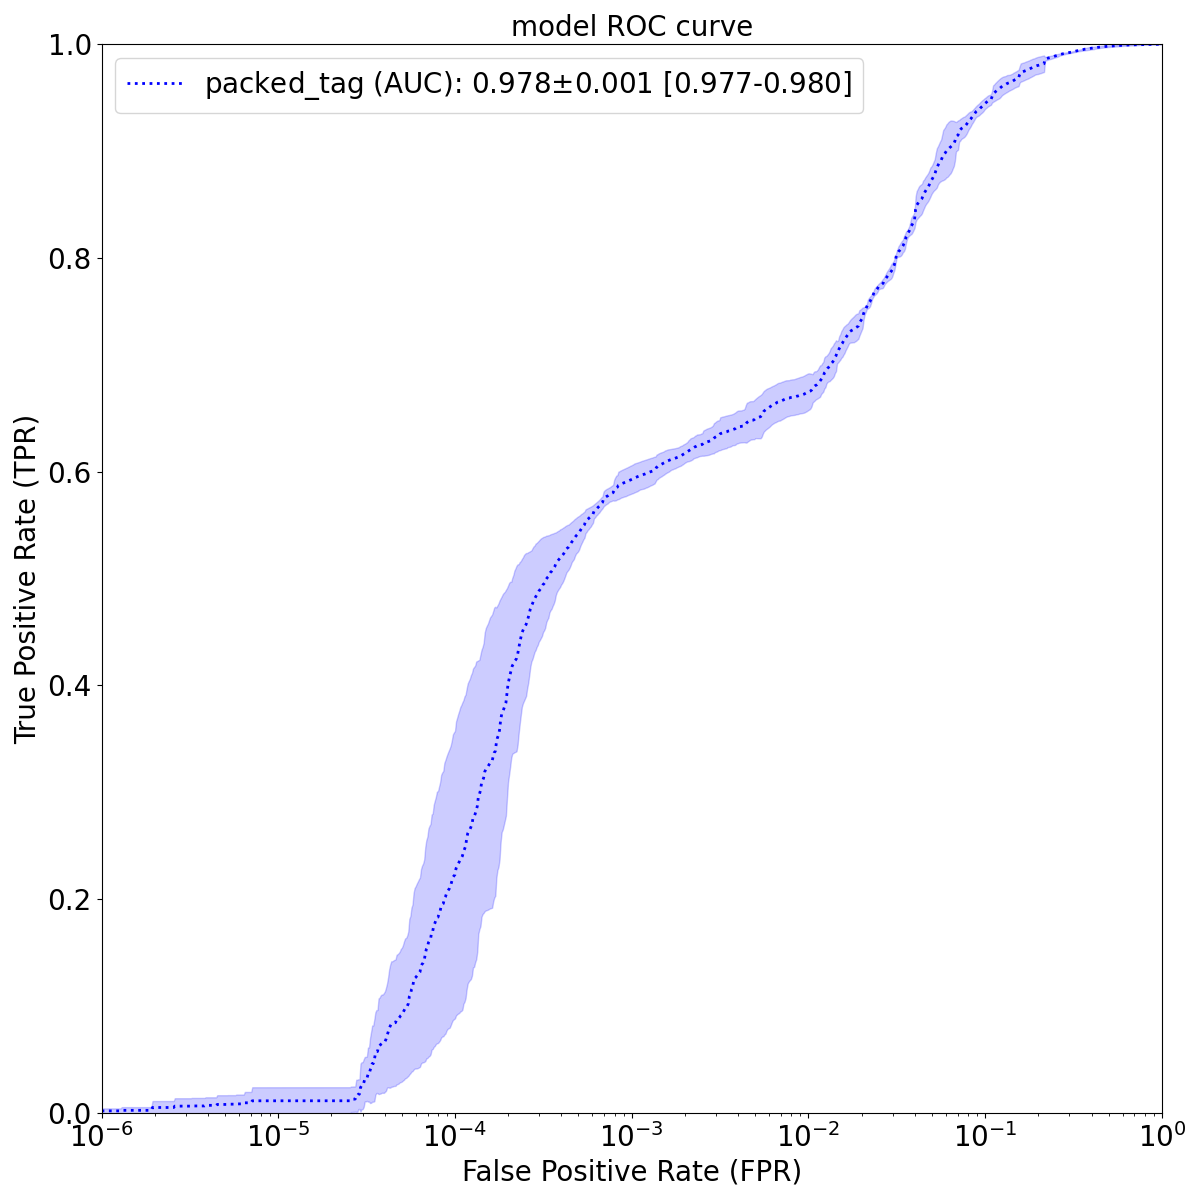
\includegraphics[width=0.6\textwidth]{./results/packed_tag_roc_aloha.png}
        \vspace*{-0.2cm}
        \caption{ROC curve and AUC statistics of \textBF{ALOHA} model for the \textbf{Packed Tag}. The line represents the \textit{mean} TPR at a given FPR, while the shaded region represents the \textit{standard deviation}. Statistics were computed over \textBF{3} training runs, each with random parameter initialization.}
        \label{fig:packedTagRocAloha}
    \end{figure}
}

\newcommand{\packedTagRocJointEmbedding}{
    \begin{figure}[H]
        \vspace*{-0.5cm}
        \centering
        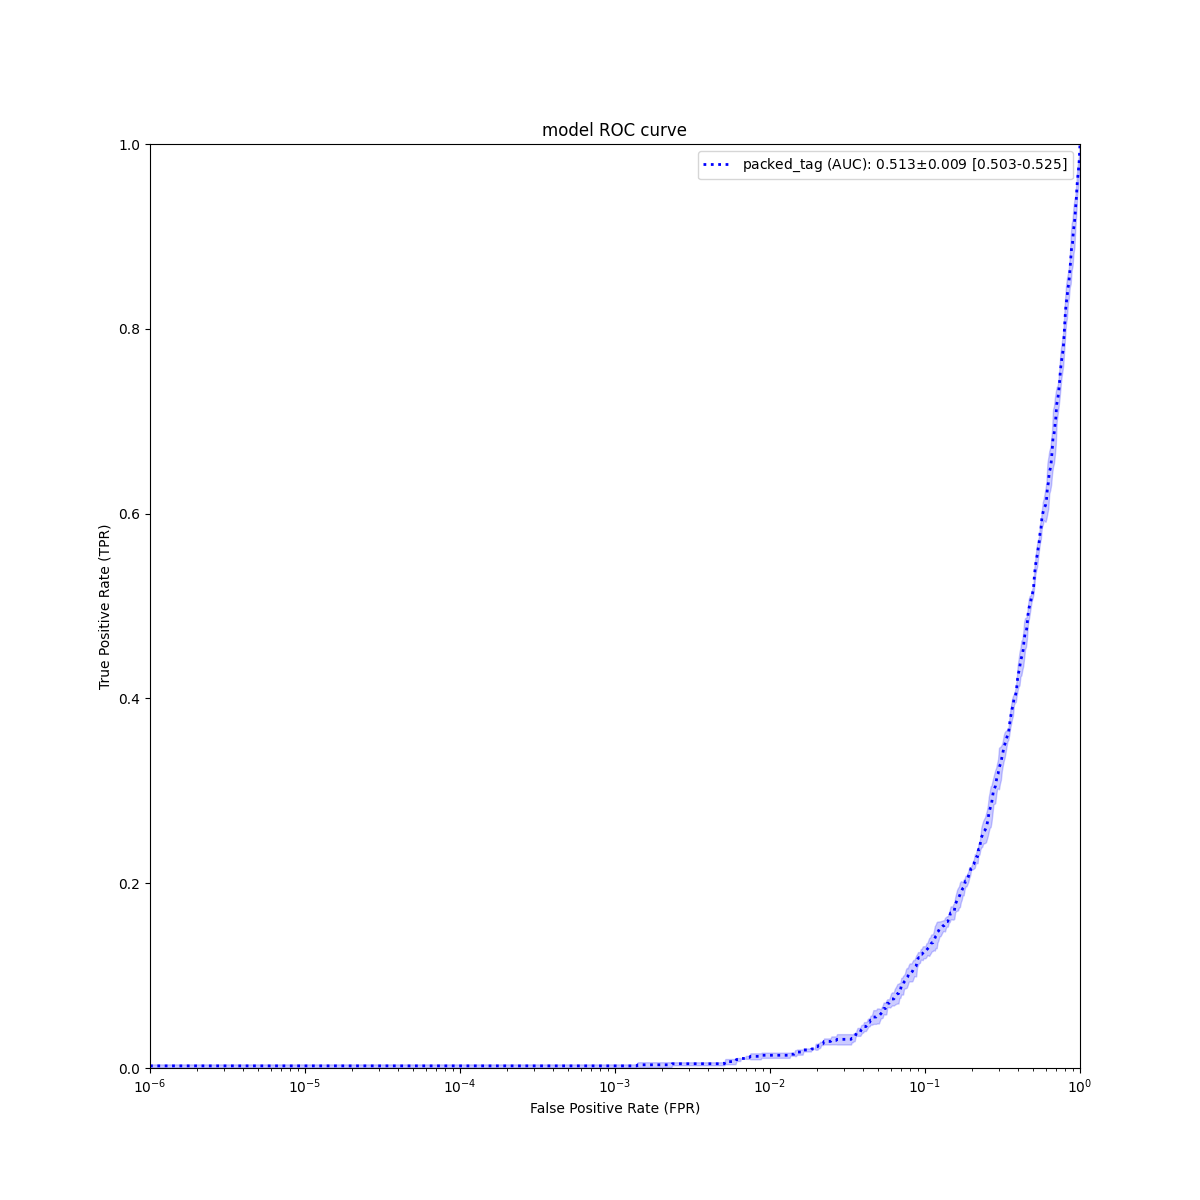
\includegraphics[width=0.6\textwidth]{./results/packed_tag_roc_jointEmbedding.png}
        \vspace*{-0.2cm}
        \caption{ROC curve and AUC statistics of \textBF{Joint Embedding} model for the \textbf{Packed Tag}. The line represents the \textit{mean} TPR at a given FPR, while the shaded region represents the \textit{standard deviation}. Statistics were computed over \textBF{3} training runs, each with random parameter initialization.}
        \label{fig:packedTagRocJointEmbedding}
    \end{figure}
}

\newcommand{\packedTagRocProposedMethod}{
    \begin{figure}[H]
        \vspace*{-0.5cm}
        \centering
        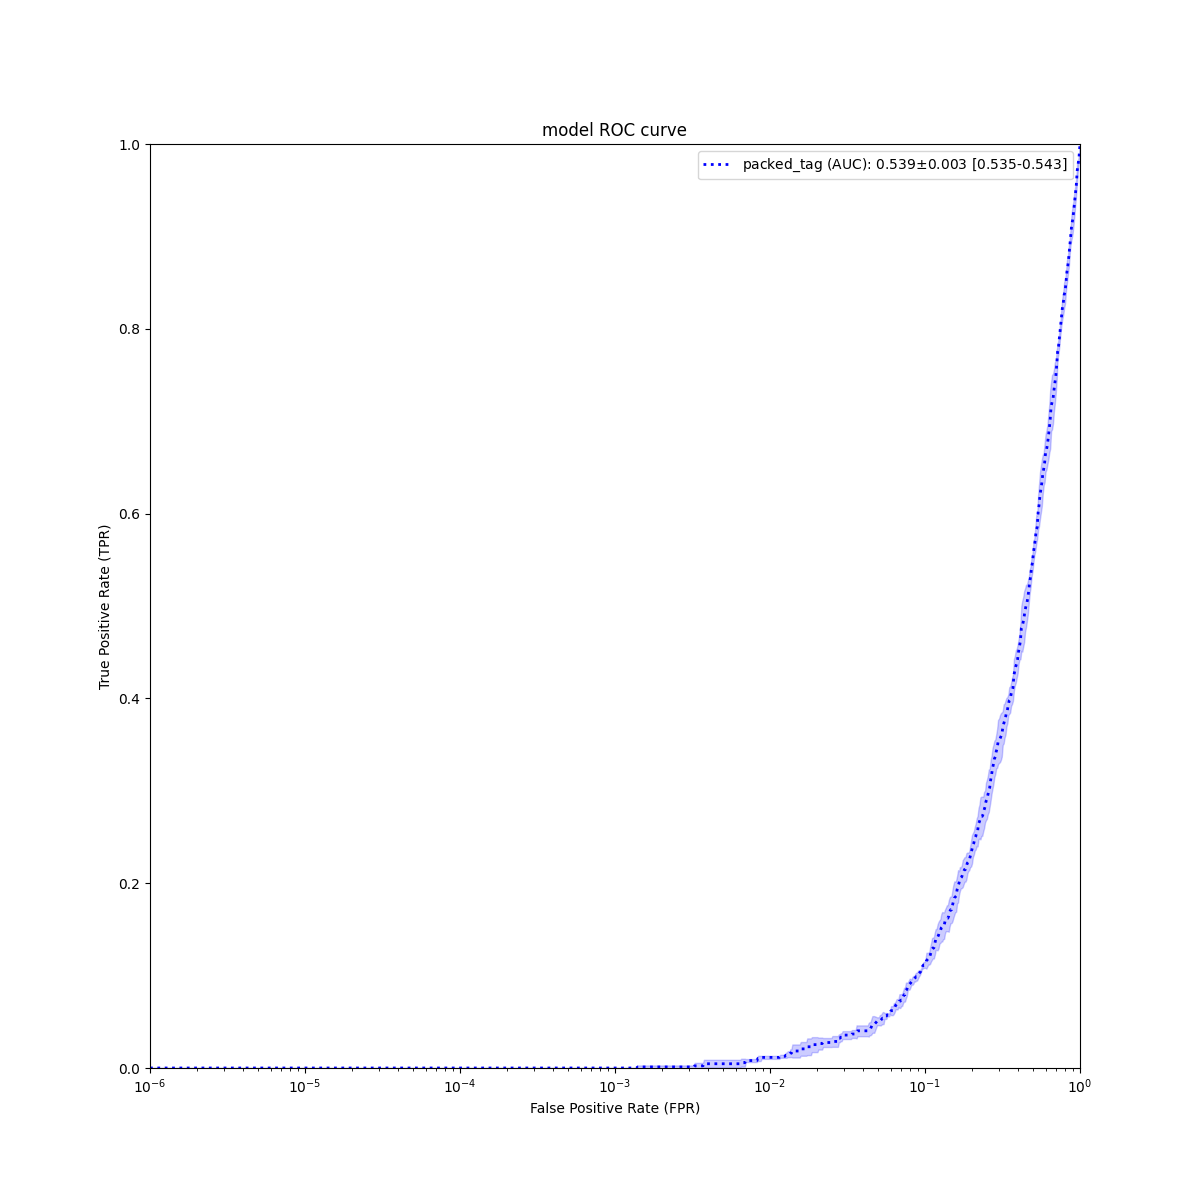
\includegraphics[width=0.6\textwidth]{./results/packed_tag_roc_proposedModel.png}
        \vspace*{-0.2cm}
        \caption{ROC curve and AUC statistics of \textBF{Proposed Model} for the \textbf{Packed Tag}. The line represents the \textit{mean} TPR at a given FPR, while the shaded region represents the \textit{standard deviation}. Statistics were computed over \textBF{3} training runs, each with random parameter initialization.}
        \label{fig:packedTagRocProposedModel}
    \end{figure}
}
